\chapter{哺乳动物的功能组织}\label{ch:b1:mammal-organization}

将解剖板上的兔子打开，首先给人的印象是
井然有序。一层肌肉质的膜，即\omterm{def:b1:mammal-organization:bodyplan}{膈肌}，把躯干分隔为胸腔
（内有心脏和两个肺）与腹腔（内有其余一切\omterm{def:b1:mammal-organization:organ}{器官}）：
其中有拳头大小的肝脏、胃、长达四米的肠道，
肠道末端是与胃一样大的盲肠，两个肾脏贴着
后壁。每个\omterm{def:b1:mammal-organization:organ}{器官}都有自己的位置、血液供应和功能，没有一个
\omterm{def:b1:mammal-organization:organ}{器官}是单独工作的。本章描述哺乳动物作为一个
有机整体是如何构成的：包括其\omterm{def:b1:mammal-organization:bodyplan}{身体构型}、\omterm{def:b1:mammal-organization:organ}{器官}所归属的系统、
细胞所处的体液区室、与外界交换物质的表面，
以及维持热平衡的机制，使其在一月份的野外
保持 \qty{39}{\celsius} 的体温。

\section{哺乳动物的身体构型}

\begin{definition}[身体构型]\label{def:b1:mammal-organization:bodyplan}
动物的\emph{身体构型}\index{身体构型}是指
其轴线、腔体与\omterm{def:b1:mammal-organization:organ}{器官}的排列方式，这种排列方式为同一类群的所有成员所共有。
哺乳动物的身体构型属于脊椎动物的构型：两侧对称，
头端带有脑和主要感觉\omterm{def:b1:mammal-organization:organ}{器官}，
（\emph{头部集中化}\index{头部集中化}），背侧为脊柱构成的轴，
包裹脊髓，具有四肢，腹侧为体腔——
即\emph{体腔}\index{体腔}，内含内脏。哺乳动物特有的是：
体腔被肌肉质的
\emph{膈肌}\index{膈肌}分隔为胸腔（内有心脏、肺），
和腹腔（内有消化\omterm{def:b1:mammal-organization:organ}{器官}、肾脏和性腺）；身体
被毛覆盖；幼体以乳汁哺育；体温
受到调节。
\end{definition}

\begin{omfigure}
\begin{tikzpicture}
  \node[anchor=south west, inner sep=0] (img) at (0,0)
    {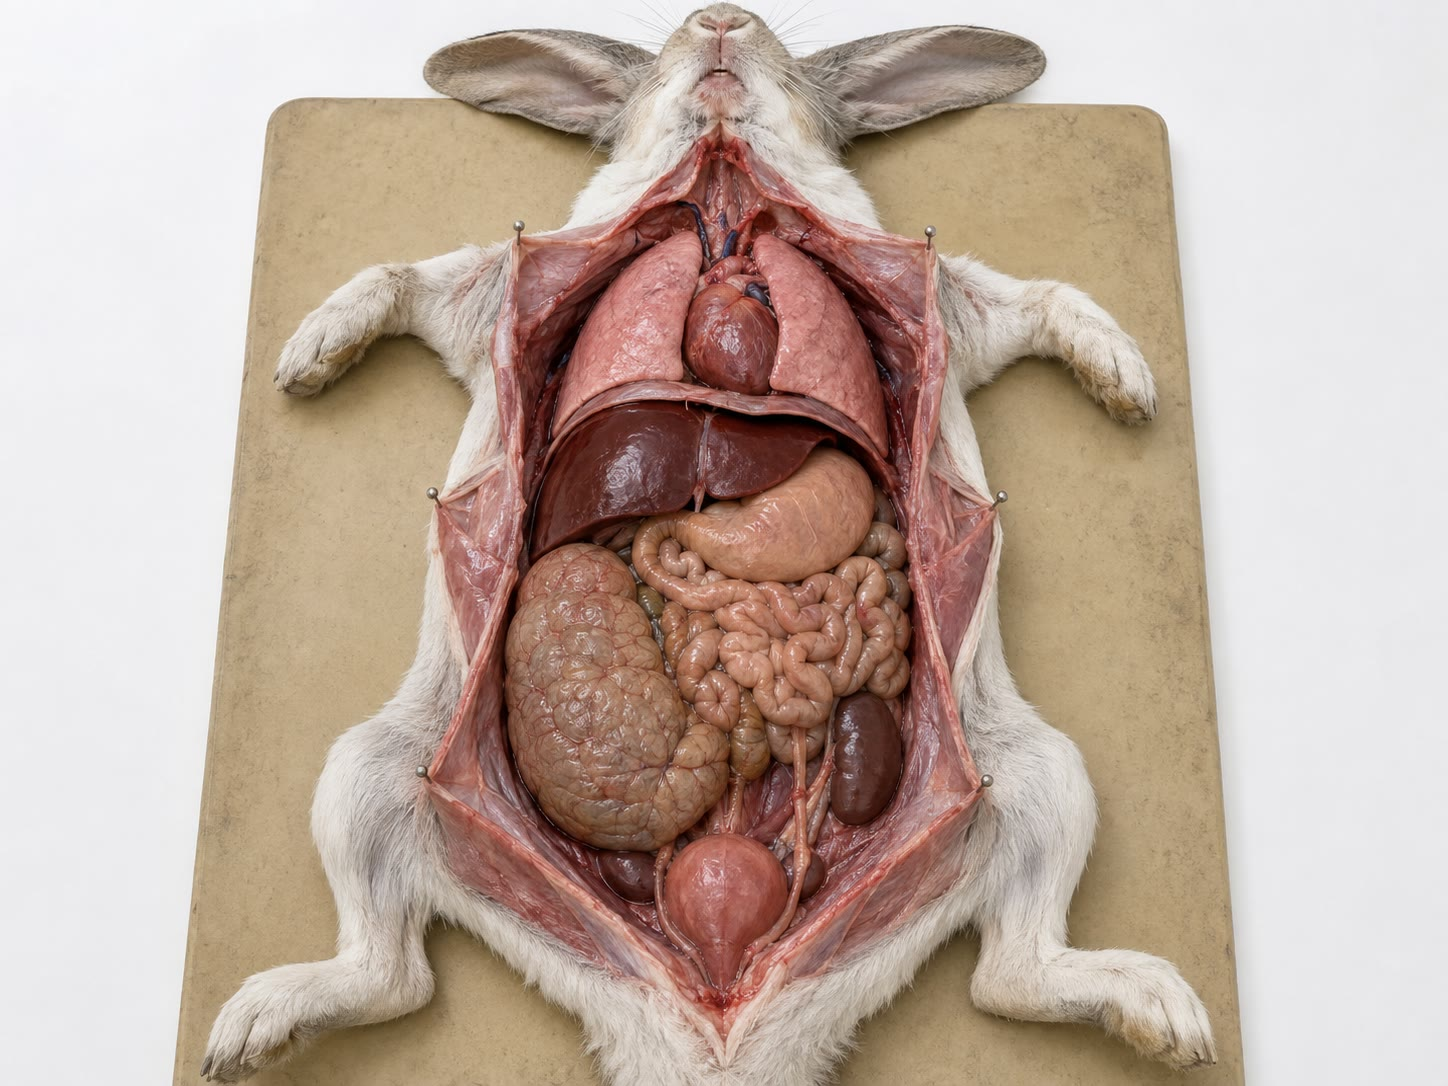
\includegraphics[width=0.6\linewidth]{images/book3/ai/fig-rabbit-dissection.jpg}};
  \begin{scope}[x={(img.south east)}, y={(img.north west)},
      every node/.style={font=\small}]
    \draw[omDef, thick] (0.44,0.72) -- (-0.02,0.90) node[left] {肺};
    \draw[omDef, thick] (0.50,0.68) -- (1.02,0.88) node[right] {心脏};
    \draw[omDef, thick] (0.53,0.61) -- (1.02,0.70) node[right] {膈肌};
    \draw[omDef, thick] (0.44,0.55) -- (-0.02,0.62) node[left] {肝脏};
    \draw[omDef, thick] (0.56,0.52) -- (1.02,0.54) node[right] {胃};
    \draw[omDef, thick] (0.52,0.42) -- (1.02,0.40) node[right] {小肠};
    \draw[omDef, thick] (0.42,0.36) -- (-0.02,0.36) node[left] {盲肠};
    \draw[omDef, thick] (0.60,0.30) -- (1.02,0.24) node[right] {肾脏};
    \draw[omDef, thick] (0.51,0.17) -- (-0.02,0.10) node[left] {膀胱};
  \end{scope}
\end{tikzpicture}

{\small 从腹侧打开的兔子。\omterm{def:b1:mammal-organization:bodyplan}{膈肌}将
胸腔（肺、心脏）与腹腔（肝脏、
胃、肠、盲肠、肾脏、膀胱）分开。每个\omterm{def:b1:mammal-organization:organ}{器官}都位于
固定位置，外包膜，并由各自的血管供血。}
\end{omfigure}

\begin{definition}[器官，器官系统]\label{def:b1:mammal-organization:organ}
\emph{器官}\index{器官}是由几种组织
（见\cref{ch:b1:body-plans-tissues}）按一定方式组织起来、执行确定功能的结构：
例如心脏泵血，肺交换气体，肾脏过滤。
\emph{器官系统}\index{器官系统}是由若干器官
协同完成某一大类功能的集合：消化系统从口腔
延伸至肛门，并附有肝脏和胰腺；循环系统由
心脏和血管组成；排泄系统由肾脏和
尿路组成。
\end{definition}

\section{器官系统及其承担的功能}

\begin{proposition}[三类功能]\label{prop:b1:mammal-organization:functions}
哺乳动物的\omterm{def:b1:mammal-organization:organ}{器官系统}承担三类功能：
\begin{itemize}
  \item \emph{营养}\index{营养功能}：摄取并
        运输物质与能量，并排出废物——
        即消化、呼吸、循环和排泄系统；
  \item \emph{联系}\index{联系功能}：感知
        \omterm{def:b1:organism-environment:organism}{环境}并对其作出反应——即感觉\omterm{def:b1:mammal-organization:organ}{器官}、神经
        系统、内分泌腺、骨骼和肌肉；
  \item \emph{生殖}\index{生殖功能}：产生
        后代——即性腺、生殖道，以及在哺乳动物中的
        乳腺。
\end{itemize}
没有哪个系统是单独工作的：每个\omterm{def:b1:mammal-organization:organ}{器官}都依赖血液供应、
依赖神经系统和内分泌系统进行协调，并依赖
骨骼和皮肤提供保护。
\end{proposition}

\begin{omfigure}
\begin{tikzpicture}[font=\footnotesize, >=Stealth, line cap=round,
  sys/.style={draw, thick, rounded corners=3pt, minimum height=7mm, minimum width=24mm, align=center, fill=white},
  lab/.style={font=\scriptsize, above},
  grp/.style={font=\small\bfseries, anchor=west}]
  \node[grp, omProp] at (0,4.6) {营养};
  \node[sys, fill=omProp!12] (dig) at (1.3,3.8) {消化};
  \node[sys, fill=omProp!12] (res) at (1.3,2.9) {呼吸};
  \node[sys, fill=omProp!12] (exc) at (1.3,2.0) {排泄};
  \node[grp, omExo] at (0,1.1) {生殖};
  \node[sys, fill=omExo!12] (gen) at (1.3,0.3) {生殖道};
  \node[sys, fill=omThm!12, minimum height=30mm] (cir) at (5.9,2.6) {循环 \\ （血液、淋巴）};
  \node[grp, omDef] at (8.6,4.6) {联系};
  \node[sys, fill=omDef!12, minimum width=30mm] (ner) at (10.3,3.8) {神经、感觉};
  \node[sys, fill=omDef!12, minimum width=30mm] (end) at (10.3,2.9) {内分泌};
  \node[sys, fill=omDef!12, minimum width=30mm] (mus) at (10.3,2.0) {骨骼、肌肉};
  \node[sys, fill=omDef!12, minimum width=30mm] (ski) at (10.3,1.1) {皮肤};
  \draw[<->, thick] (dig.east) -- (cir.west |- dig.east) node[lab, midway] {营养物质};
  \draw[<->, thick] (res.east) -- (cir.west |- res.east) node[lab, midway] {$\mathrm{O_2}$, $\mathrm{CO_2}$};
  \draw[<->, thick] (exc.east) -- (cir.west |- exc.east) node[lab, midway] {废物};
  \draw[<->, thick] (gen.east) -- ++(1.6,0) |- (cir.south west);
  \draw[<->, thick] (cir.east |- ner.west) -- (ner.west);
  \draw[<->, thick] (cir.east |- end.west) -- (end.west) node[lab, midway] {激素};
  \draw[<->, thick] (cir.east |- mus.west) -- (mus.west);
  \draw[<->, thick] (cir.south east) -| ++(0.5,0) |- (ski.west);
\end{tikzpicture}

{\small 哺乳动物的\omterm{def:b1:mammal-organization:organ}{器官系统}按功能分组。
循环是中枢：每个系统都与血液交换物质，并且
血液将一个系统摄入的物质运送给所有其他系统。}
\end{omfigure}

\begin{example}[一口草料]\label{ex:b1:mammal-organization:mouthful}
兔子吃的草先由门齿切断，再由臼齿磨碎
（骨骼与肌肉），经品尝和嗅闻（感觉），随后吞咽，
在胃和小肠中被消化；其中的糖类与氨基酸
穿过肠壁进入血液并抵达肝脏，肝脏
在激素调控下储存或释放它们（内分泌）；其
纤维素在盲肠中被细菌发酵；用于氧化糖类的
氧经肺摄入，二氧化碳也经同一途径排出，
氨基酸生成的尿素经肾脏排出，整个过程产生的热量
经皮肤散失。这一口草料共涉及
七个系统。
\end{example}

\section{身体的体液分区}

\begin{definition}[体液分区]\label{def:b1:mammal-organization:compartments}
水约占哺乳动物质量的 \qty{60}{\%}。其中三分之二为
\emph{细胞内液}\index{细胞内液}，位于细胞内；
三分之一为\emph{细胞外液}\index{细胞外液}，
即在\cref{ch:b1:organism-environment}中所述的\omterm{def:b1:organism-environment:milieu}{内环境}，本身
又分为\emph{组织液}\index{组织液}，
包围细胞（占其四分之三）以及
\emph{血浆}\index{血浆}位于血管内（占其四分之一）。\emph{淋巴液}\index{淋巴液}
是由淋巴管收集的组织液，
回流至血液。两种细胞外液的
成分几乎相同——血浆的不同之处在于其蛋白质，它们不能穿过
毛细血管壁——二者都与细胞内液差别显著。
\end{definition}

\begin{omfigure}
\begin{tikzpicture}[font=\small, line cap=round]
  \draw[thick, fill=gray!8, rounded corners=6pt] (0,0) rectangle (11.6,4.6);
  \node[anchor=north west, font=\small\bfseries] at (0.15,4.55) {体内总水量：\qty{42}{L}（\qty{60}{\%} 占 \qty{70}{kg}）};
  \draw[thick, fill=omDef!14, rounded corners=5pt] (0.3,0.3) rectangle (6.4,3.8);
  \node[anchor=north west, align=left] at (0.4,3.7) {\textbf{细胞内液}：\qty{28}{L}\\ 高 $\mathrm{K^+}$（\qty{140}{mmol/L}），\\ 磷酸基团、蛋白质；\\ 低 $\mathrm{Na^+}$（\qty{10}{mmol/L}）};
  \draw[thick, fill=omProp!14, rounded corners=5pt] (6.7,0.3) rectangle (11.3,3.8);
  \node[anchor=north west, align=left] at (6.8,3.7) {\textbf{细胞外液}：\qty{14}{L}\\ 高 $\mathrm{Na^+}$（\qty{140}{mmol/L}），\\ $\mathrm{Cl^-}$、$\mathrm{HCO_3^-}$};
  \draw[thick, fill=omProp!30, rounded corners=4pt] (6.9,0.45) rectangle (9.2,1.55);
  \node[align=center, font=\footnotesize] at (8.05,1.0) {组织液 \\ \qty{11}{L}};
  \draw[thick, fill=omThm!30, rounded corners=4pt] (9.4,0.45) rectangle (11.1,1.55);
  \node[align=center, font=\footnotesize] at (10.25,1.0) {血浆 \\ \qty{3}{L}};
\end{tikzpicture}

{\small \qty{70}{kg} 成人的体液分区。其中三分之二
的水位于细胞内；细胞外的三分之一，
在\omterm{def:b1:mammal-organization:compartments}{组织液}与\omterm{def:b1:mammal-organization:compartments}{血浆}之间分配，构成\omterm{def:b1:organism-environment:milieu}{内环境}。
细胞外以钠离子为主，细胞内以钾离子为主——这一差异，每个细胞
都要消耗能量加以维持（见\cref{ch:b1:membranes-transport}）。}
\end{omfigure}

\begin{method}[用稀释法测量体液分区]\label{met:b1:mammal-organization:dilution}
\begin{enumerate}
  \item 选择一种只分布于该分区而不分布于其他任何地方的标记物：
        与\omterm{def:b1:mammal-organization:compartments}{血浆}蛋白结合的染料（埃文斯蓝），用于测定\omterm{def:b1:mammal-organization:compartments}{血浆}；
        菊粉是一种糖，能离开血管但
        不进入细胞，用于测定\omterm{def:b1:mammal-organization:compartments}{细胞外液}；重水
        用于测定体内总水量。
  \item 注入已知量 $m$，并等待充分混合（\omterm{def:b1:mammal-organization:compartments}{血浆}需数分钟，
        总水量需数小时）。
  \item 测定\omterm{def:b1:mammal-organization:compartments}{血浆}样本中的浓度 $c$，并校正
        等待期间的任何损失（尿液排出、代谢）。
  \item 体积为 $V = m/c$。\omterm{def:b1:mammal-organization:compartments}{细胞内液}体积等于总水量
        减去\omterm{def:b1:mammal-organization:compartments}{细胞外液}体积；\omterm{def:b1:mammal-organization:compartments}{组织液}体积等于\omterm{def:b1:mammal-organization:compartments}{细胞外液}减去
        \omterm{def:b1:mammal-organization:compartments}{血浆}体积。血容量等于\omterm{def:b1:mammal-organization:compartments}{血浆}体积除以血液中的
        \omterm{def:b1:mammal-organization:compartments}{血浆}比例（$1 - $ 红细胞压积）。
\end{enumerate}
\end{method}

\begin{example}[血浆体积]\label{ex:b1:mammal-organization:evansblue}
将 \qty{50}{mg} 埃文斯蓝注入一名 \qty{70}{kg} 男子体内，
十分钟后测得\omterm{def:b1:mammal-organization:compartments}{血浆}浓度为 \qty{16.7}{mg/L}：
$V = 50/16.7 = \qty{3.0}{L}$，即\omterm{def:b1:mammal-organization:compartments}{血浆}体积。若红细胞压积为
\qty{45}{\%}，则血液体积为 $3.0/0.55 = \qty{5.5}{L}$——
\qty{8}{\%} 的体重，这一比例从小鼠到
鲸都成立。
\end{example}

\section{交换表面与循环}

\begin{proposition}[每个交换表面都与血液相连]\label{prop:b1:mammal-organization:surfaces}
哺乳动物通过四个表面与外界交换物质，这些表面均向体内折叠，
并由致密的毛细血管网灌注：其中
肠黏膜（人体内为 \qty{30}{m^2}）负责营养物质和水的吸收，
肺泡表面（\qty{100}{m^2}）负责氧气和
二氧化碳的交换，肾脏的滤过表面（一百万个
肾小球，每天滤过 \qty{180}{L} \omterm{def:b1:mammal-organization:compartments}{血浆}）负责废物排出和
\omterm{def:b1:organism-environment:milieu}{内环境}的调节，皮肤（\qty{2}{m^2}）负责
散热和少量水分的散失。循环将它们联系起来：离开一个表面的血液
一分钟内即可到达下一个表面，因此经肠道吸收的物质
被来自肺的氧气所氧化，其废物
经肾脏排出。
\end{proposition}

\begin{omfigure}
\begin{tikzpicture}[font=\small, >=Stealth, line cap=round,
  org/.style={draw, thick, rounded corners=4pt, minimum height=8mm, minimum width=22mm, align=center, fill=white}]
  \node[org, fill=omDef!12] (lung) at (0,3.2) {肺 \\ \qty{100}{m^2}};
  \node[org, fill=omThm!15, minimum width=26mm, minimum height=12mm] (heart) at (0,0) {心脏 \\ 右 $\mid$ 左};
  \node[org, fill=omProp!12] (gut) at (5.2,1.6) {肠道 \\ \qty{30}{m^2}};
  \node[org, fill=omProp!12] (liver) at (5.2,0.0) {肝脏};
  \node[org, fill=omProp!12] (kid) at (5.2,-1.6) {肾脏 \\ \qty{180}{L/d}};
  \node[org, fill=omExo!12] (mus) at (5.2,3.2) {肌肉、皮肤、\\ 脑及其他};
  % pulmonary loop
  \draw[->, very thick, omDef] (heart.north west) ++(-0.2,0) |- (lung.west) node[pos=0.25, left, font=\footnotesize, align=right] {肺 \\ 循环};
  \draw[->, very thick, omThm] (lung.east) -| ($(heart.north east)+(0.2,0)$);
  % systemic loop: left heart -> organs (parallel) -> right heart
  \draw[very thick, omThm] (heart.east) -- ++(1.2,0) coordinate (a);
  \draw[->, very thick, omThm] (a) |- (mus.west);
  \draw[->, very thick, omThm] (a) |- (gut.west);
  \draw[->, very thick, omThm] (a) |- (kid.west);
  \draw[->, very thick, omThm] (a) -- (liver.west);
  \draw[->, very thick, omDef] (gut.south) -- (liver.north) node[midway, right, font=\footnotesize] {门静脉};
  \coordinate (b) at (8.0,0.8);
  \draw[very thick, omDef] (mus.east) -| (b);
  \draw[very thick, omDef] (liver.east) -| (b);
  \draw[very thick, omDef] (kid.east) -| (b);
  \draw[->, very thick, omDef] (b) |- ++(0,-3.2) -| (heart.south) node[pos=0.25, below, font=\footnotesize] {体循环：静脉};
\end{tikzpicture}

{\small 哺乳动物的双循环。右心将含氧少的血液（蓝色）
送入肺部；左心将含氧的血液（红色）送入各\omterm{def:b1:mammal-organization:organ}{器官}，
各\omterm{def:b1:mammal-organization:organ}{器官}并联排列，因此每个\omterm{def:b1:mammal-organization:organ}{器官}都能获得新鲜的动脉血。
来自消化道的血液先经过肝脏，
再回到心脏。}
\end{omfigure}

\begin{omfigure}
\begin{tikzpicture}
\begin{axis}[
  xbar, bar width=8pt,
  width=0.82\linewidth, height=6.2cm,
  axis x line=bottom, axis y line=left,
  xmin=0, xmax=1.8, xlabel={静息时血流量（\unit{L/min}）},
  xlabel style={font=\small, at={(axis description cs:0.5,-0.13)}, anchor=north},
  symbolic y coords={heart muscle, skin, brain, skeletal muscle, kidneys, liver and gut},
  ytick=data, yticklabels={心肌, 皮肤, 脑, 骨骼肌, 肾, 肝和肠}, tick label style={font=\small},
  enlarge y limits=0.12, xtick={0,0.5,1.0,1.5},
  nodes near coords, nodes near coords style={font=\scriptsize, anchor=west},
]
\addplot[fill=omThm!45, draw=omThm] coordinates
  {(0.25,heart muscle) (0.4,skin) (0.75,brain) (1.0,skeletal muscle) (1.1,kidneys) (1.35,liver and gut)};
\end{axis}
\end{tikzpicture}

{\small 人体静息时心输出量 \qty{5}{L/min} 在各\omterm{def:b1:mammal-organization:organ}{器官}间的分配。
肾脏占体重的 \qty{0.5}{\%}，却获得约五分之一的血液——
这是为每天将全部\omterm{def:b1:mammal-organization:compartments}{血浆}过滤
约六十次所付出的代价。运动时，肌肉的分配比例升至原来的十倍，
而消化道的分配比例则下降。}
\end{omfigure}

\begin{example}[循环时间]\label{ex:b1:mammal-organization:circtime}
若血液量为 \qty{5.5}{L}，心输出量为 \qty{5}{L/min}，
一滴血液在静息时约一分钟即可完成一次双循环，
剧烈运动时则约为其四分之一，此时心输出量升至
\qty{20}{L/min}。心输出量与 $M^{3/4}$ 成比例
（见\cref{thm:b1:organism-environment:kleiber}）：一只 \qty{2}{kg} 的兔子，
心输出量约为 \qty{0.35}{L/min}，血液量为 \qty{160}{mL}——两者循环时间
大致相同（相差不超过两倍），心率为
每分钟 \qty{200}{} 次搏动。
\end{example}

\section{内温性与热平衡}

\begin{proposition}[热量收支]\label{prop:b1:mammal-organization:heatbudget}
\index{热量收支}
处于稳定体温的哺乳动物满足
\[
M - W = R + C + K + E ,
\]
其中 $M$ 为代谢产热，$W$ 为对外做的机械功，
等式右边为各项散热：辐射散热 $R$、
对空气的对流散热 $C$、对地面的传导散热 $K$，以及蒸发散热
$E$（来自肺部，以及汗液或喘息）。前三项散热
与 $T_b - T_a$ 成正比，并受皮毛隔热
和流向皮肤的血流量支配；蒸发则是空气温度高于体温时唯一有效的散热途径。
若该等式不成立，
体温的变化速率由这一失衡
及身体的热容决定（约为
\qty{3.5}{kJ.kg^{-1}.K^{-1}}）。
\end{proposition}
\begin{proof}
对身体在一段体温不变的时间内应用能量守恒：
即释放的化学能（$M$）
以功或热的形式经四个物理途径离开。
$R$、$C$、$K$ 与温差成正比，
这是牛顿冷却定律（见\cref{ch:b1:organism-environment}）；
$E$ 与该温差无关，是因为蒸发
由湿度梯度而非温度梯度驱动。
\end{proof}

\begin{omfigure}
\begin{tikzpicture}[font=\small, >=Stealth, line cap=round]
  \draw[very thick, fill=omThm!8, rounded corners=16pt] (0,0) rectangle (5.0,3.0);
  \node[align=center] at (2.5,1.5) {体核 \qty{39}{\celsius}\\ 产热 $M$\\（基础代谢、战栗、活动）};
  \draw[->, very thick, omThm] (5.0,2.5) -- (6.6,2.5) node[right, align=left] {$R$：向墙壁与天空辐射};
  \draw[->, very thick, omThm] (5.0,1.8) -- (6.6,1.8) node[right, align=left] {$C$：对空气的对流};
  \draw[->, very thick, omThm] (5.0,1.1) -- (6.6,1.1) node[right, align=left] {$K$：对地面的传导};
  \draw[->, very thick, omDef] (5.0,0.4) -- (6.6,0.4) node[right, align=left] {$E$：蒸发（呼吸、汗液）};
  \draw[->, very thick, omExo] (-1.6,1.5) -- (0,1.5) node[pos=0, left, align=right] {食物能量 \\（以及储存的脂肪）};
  \draw[->, very thick, gray] (2.5,0) -- (2.5,-0.9) node[below, align=center] {$W$：对外做功};
  \node[font=\footnotesize, align=center, anchor=south] at (2.5,3.1) {皮毛与皮肤血流决定 $R$、$C$、$K$；\\ 它们 $\propto (T_b - T_a)$};
\end{tikzpicture}

{\small \omterm{prop:b1:organism-environment:thermo}{内温动物}的热量收支。产热必须等于四项散热之和
加上对外做功；动物通过调节产热
（战栗、活动）、隔热（皮毛、姿势、皮肤血流）
和蒸发来维持平衡。}
\end{omfigure}

\begin{proposition}[体温调节的方式]\label{prop:b1:mammal-organization:thermoreg}
面对寒冷，哺乳动物一方面减少散热——如竖起皮毛、
收缩皮肤和四肢的血管、蜷缩身体、聚集成群——并
增加产热：战栗（肌肉的节律性收缩），
以及在小型和幼年哺乳动物中发生的\emph{非战栗产热}\index{非战栗产热}，
其产热部位是\emph{棕色脂肪组织}\index{棕色脂肪组织}，
其线粒体将脂肪中的能量直接以热的形式释放。
面对温暖，哺乳动物扩张皮肤血管
（兔子的耳朵可散去三分之一的热量），并通过
出汗（马、人）或喘息（狗、兔子）蒸发水分。这一切都
由下丘脑调控，它设定\omterm{def:b1:organism-environment:homeostasis}{调定点}，并读取
血液和皮肤的温度。
\end{proposition}
\begin{proof}[证据]
用植入的探针加热狗的下丘脑，会使其
在寒冷的房间中喘息并扩张皮肤血管；冷却探针
则使其在温暖的房间中战栗。将大鼠置于
\qty{5}{\celsius} \omterm{def:b1:organism-environment:organism}{环境}中，其耗氧量一小时内增至三倍，
增量的一半来自战栗（以肌肉的电活动记录），另一半来自棕色
脂肪，用热电偶测得其温度高于
周围组织。红外图像显示，兔子在
\qty{30}{\celsius} \omterm{def:b1:organism-environment:organism}{环境}中耳朵温度接近体温，在
\qty{5}{\celsius} \omterm{def:b1:organism-environment:organism}{环境}中则接近气温。
\end{proof}

\begin{example}[兔子的耳朵]\label{ex:b1:mammal-organization:ears}
两只耳朵各约 \qty{50}{cm^2}，薄而几乎无毛，血管丰富，
血管开放、温度为 \qty{30}{\celsius}，置于
\qty{20}{\celsius} 的空气中，裸皮系数为
\qty{10}{W.m^{-2}.K^{-1}}，则散热为 $10\times 0.01\times 10 =
\qty{1}{W}$，约为静息兔子产热量的六分之一。
当 \qty{5}{\celsius} 时，血管收缩，耳朵冷却至
接近气温，经耳朵的散热降至 \qty{0.2}{W} 以下。
\end{example}

\begin{remark}[协调]\label{rem:b1:mammal-organization:coordination}
上述每一项调节——血管收缩、肌肉战栗、
腺体分泌——都是经神经或激素传递的指令。
神经系统沿固定线路在毫秒内起作用；内分泌系统
则通过血液在数分钟至数小时内起作用，到达每一个
带有相应受体的细胞。其机制是
本科二年级分册的内容，本学年暂将其视为已知，研究它们所
协调的对象。
\end{remark}

\section{练习}

\begin{exercise}[$\star$]\label{exo:b1:mammal-organization:1}
列出哺乳动物\omterm{def:b1:mammal-organization:bodyplan}{身体构型}中与所有脊椎动物共有的特征，
以及哺乳动物所特有的特征。
\end{exercise}

\begin{exercise}[$\star$]\label{exo:b1:mammal-organization:2}
将每个\omterm{def:b1:mammal-organization:organ}{器官系统}归入三类功能之一，
并说出每个系统中的一个\omterm{def:b1:mammal-organization:organ}{器官}。
\end{exercise}

\begin{exercise}[$\star$]\label{exo:b1:mammal-organization:3}
一名 \qty{60}{kg} 的女性：估算其总体水、\omterm{def:b1:mammal-organization:compartments}{细胞内
液}与\omterm{def:b1:mammal-organization:compartments}{细胞外液}的体积、\omterm{def:b1:mammal-organization:compartments}{组织液}的体积及
\omterm{def:b1:mammal-organization:compartments}{血浆}体积。
\end{exercise}

\begin{exercise}[$\star$]\label{exo:b1:mammal-organization:4}
根据血流图，心输出量中有多大比例流向
肾脏，全部血量（
\qty{5.5}{L}）每天被泵经肾脏多少次？
\end{exercise}

\begin{exercise}[$\star\star$]\label{exo:b1:mammal-organization:5}
向一名 \qty{70}{kg} 的男子注射 \qty{2.0}{g} 菊糖；
混合后，且尿中已损失 \qty{0.3}{g} 后，\omterm{def:b1:mammal-organization:compartments}{血浆}
浓度为 \qty{0.12}{g/L}。计算\omterm{def:b1:mammal-organization:compartments}{细胞外液}体积，
并在总体水为 \qty{42}{L} 的条件下，计算\omterm{def:b1:mammal-organization:compartments}{细胞内液}体积。
\end{exercise}

\begin{exercise}[$\star\star$]\label{exo:b1:mammal-organization:6}
解释为何\omterm{def:b1:mammal-organization:compartments}{血浆}与\omterm{def:b1:mammal-organization:compartments}{组织液}的离子
组成相同而蛋白质含量不同，并说明若\omterm{def:b1:mammal-organization:compartments}{血浆}蛋白
丢失，\omterm{def:b1:mammal-organization:compartments}{组织液}体积将如何变化。
\end{exercise}

\begin{exercise}[$\star\star$]\label{exo:b1:mammal-organization:7}
为何体循环中的各\omterm{def:b1:mammal-organization:organ}{器官}是并联而非
串联排列？若将脑置于肌肉下游，会产生
什么后果？
\end{exercise}

\begin{exercise}[$\star\star$]\label{exo:b1:mammal-organization:8}
一名静息的人（$M = \qty{80}{W}$，$W = 0$）处于
\qty{20}{\celsius} 的空气中，经肺与
皮肤蒸发散失 \qty{20}{W}。若辐射、对流与传导三者合计为
$hS(T_b - T_a)$，其中 $S = \qty{1.8}{m^2}$，皮肤温度 $T_b$ $=
\qty{33}{\celsius}$，求 $h$。当空气温度
达到 \qty{33}{\celsius} 时，皮肤温度会如何变化？
\end{exercise}

\begin{exercise}[$\star\star$]\label{exo:b1:mammal-organization:9}
一名运动中的人产热 \qty{800}{W}，并做外功 \qty{200}{W}，
非蒸发散热为 \qty{150}{W}。为使体温保持稳定，
每小时须蒸发多少水（潜热为
\qty{2.4}{kJ/g}）？若停止出汗，体温以多快的速率
上升（\qty{70}{kg}，\qty{3.5}{kJ.kg^{-1}.K^{-1}}）？
\end{exercise}

\begin{exercise}[$\star\star\star$]\label{exo:b1:mammal-organization:10}
新生哺乳动物与小型物种依靠棕色脂肪
而非战栗。请结合表面积与体积之比及
各机制的性质，提出两点理由。
\end{exercise}

\begin{exercise}[$\star\star\star$]\label{exo:b1:mammal-organization:11}
一只狗坐在寒冷的房间中，用探针加热其下丘脑，
请预测其反应，以及一
小时后的体核温度。随后请预测下丘脑已被破坏的狗
先后置于寒冷与炎热房间中的反应。
\end{exercise}

\begin{exercise}[$\star\star\star$]\label{exo:b1:mammal-organization:12}
“\omterm{def:b1:organism-environment:milieu}{内环境}是哺乳动物私有的海洋。”请以一段文字
讨论这一比喻：\omterm{def:b1:mammal-organization:compartments}{细胞外液}是什么，什么
使其保持恒定，哪些\omterm{def:b1:mammal-organization:organ}{器官系统}是它的海岸。
\end{exercise}

\section{问题：兔子的一天}

\begin{problem}[{周末问题——一只两千克兔子在一月份的二十四小时：
其能量、水分、血液与
热量，最后归结为每日能量消耗与水的周转}]
\label{pb:b1:mammal-organization:1}
一只野生兔子质量为 \qty{2.0}{kg}，体温为
\qty{39}{\celsius}。其\omterm{def:b1:organism-environment:allometry}{基础代谢率}服从\omterm{thm:b1:organism-environment:kleiber}{克莱伯定律}，
$B = \qty{3.4}{W}\,(M/\qty{1}{kg})^{3/4}$。其一天的安排：\qty{12}{h} 静息
于洞穴中，处于其\omterm{prop:b1:organism-environment:thermo}{热中性区}内，\qty{6}{h} 以
\omterm{def:b1:organism-environment:allometry}{基础代谢率}的三倍觅食，另有 \qty{6}{h} 在
外面静息，\omterm{def:b1:organism-environment:organism}{环境}为 \qty{5}{\celsius}，须产热为\omterm{def:b1:organism-environment:allometry}{基础代谢率}的两倍。它
食用含 \qty{25}{\%} 干物质的新鲜草，其干物质
含能 \qty{18}{kJ/g}，其中可消化 \qty{65}{\%}。

\medskip
\noindent\textbf{第一部分——能量。}
\begin{enumerate}
  \item 计算兔子的\omterm{def:b1:organism-environment:allometry}{基础代谢率}，单位为瓦特。
  \item 计算三个时段中各自消耗的能量，单位为
        千焦。
  \item 计算每日能量消耗，并将其表示为
        \qty{24}{h} 内\omterm{def:b1:organism-environment:allometry}{基础代谢率}的倍数。
  \item 计算一克新鲜草的可消化能量。
  \item 计算每日所食新鲜草的质量，以及其
        所含干物质的质量。
  \item 将新鲜草的摄入量表示为体重的分数。
  \item 取每消耗一升氧气对应 \qty{20}{kJ} 的换算关系，计算
        每日耗氧量，以及以毫升每
        分钟计的平均速率。
  \item 呼吸商为 $0.9$（$\mathrm{CO_2}$ 的升数与
        $\mathrm{O_2}$ 的升数之比），计算每日二氧化碳排出量，
        分别以升和克表示
        （\qty{22.4}{L/mol}，\qty{44}{g/mol}）。
\end{enumerate}

\medskip
\noindent\textbf{第二部分——水。}
氧化已消化的干物质可产生代谢水，每克干物质产生 \qty{0.6}{g}
的代谢水。未消化的干物质随粪便排出，粪便
含水 \qty{40}{\%}。每日尿量为 \qty{130}{mL}。兔子
每日呼吸 \qty{860}{L} 空气，吸入的空气温度为 \qty{10}{\celsius}，
含水汽 \qty{5}{g/m^3}，呼出空气在
\qty{37}{\celsius} 时饱和，含水汽 \qty{44}{g/m^3}。经皮肤的蒸发量
为每日 \qty{20}{g}。
\begin{enumerate}[resume]
  \item 计算随草摄入的水量。
  \item 计算产生的代谢水量。
  \item 计算粪便的质量，以及粪便带走的水量。
  \item 计算呼吸丢失的水量。
  \item 列出水的平衡：总输入、总输出及其
        差值。
  \item 兔子是否必须饮水？差值去向如何？
  \item 八月份草中干物质占 \qty{50}{\%}。重新计算
        能量摄入相同时食物中的水量，并作出结论。
\end{enumerate}

\medskip
\noindent\textbf{第三部分——血液与体液分区。}
\begin{enumerate}[resume]
  \item 利用本章给出的比例，计算兔子的体总水量、
        \omterm{def:b1:mammal-organization:compartments}{细胞外液}体积及\omterm{def:b1:mammal-organization:compartments}{血浆}体积。
  \item 注射 \qty{1.5}{mg} 埃文斯蓝，混合后\omterm{def:b1:mammal-organization:compartments}{血浆}
        浓度为 \qty{15}{mg/L}。计算
        \omterm{def:b1:mammal-organization:compartments}{血浆}体积，并与估算值比较。
  \item 已知红细胞比容为 \qty{40}{\%}，计算血液体积。
  \item 心输出量按 $M^{3/4}$ 标度变化，人的值为
        \qty{70}{kg} 时 \qty{5}{L/min}。计算兔子的心输出量
        以及一滴血液完成一次
        循环所需的时间。
  \item 心率为每分钟 \qty{200}{} 次搏动，计算
        每搏输出量。
\end{enumerate}

\medskip
\noindent\textbf{第四部分——热量。}
兔子的体表面积为 $S = \qty{0.1}{m^2}\,(M/\qty{1}{kg})^{2/3}$；
其皮毛的传热系数为 $h = \qty{2.5}{W.m^{-2}.K^{-1}}$；每只耳朵为
\qty{50}{cm^2} 的近裸皮肤，其 $h = \qty{10}{W.m^{-2}.K^{-1}}$。
\begin{enumerate}[resume]
  \item 计算兔子的体表面积。
  \item 计算在 \qty{5}{\celsius} 时经皮毛散失的热量，并
        与假定的户外时段产热量比较。
  \item 计算两耳经血管开放时的散热量
        （皮肤温度为 \qty{39}{\celsius}），以及血管关闭时
        （皮肤温度为 \qty{8}{\celsius}）的散热量。一月份兔子如何应对？
  \item 八月份，在 \qty{30}{\celsius} 时，计算经
        皮毛及开放耳朵的散热量，并将二者之和与
        基础产热量比较。兔子如何保持
        \qty{39}{\celsius} 的体温？
  \item 给出结果：兔子每日能量消耗以兆焦计，
        表示为其\omterm{def:b1:organism-environment:allometry}{基础代谢率}的倍数；每日水的周转量以克计，
        并表示为其体重的分数。
\end{enumerate}
\end{problem}
